%!TEX root = ../dissertation.tex
\chapter{Research method}
\label{chap:method}
% Describe collection of data from SWORDS, automated labelling of employees, manual labelling of repos, exploratory data analysis
We conducted an exploratory data analysis to gather more insights into the research software landscape \cite{tukey_exploratory_1977}. The study is based on a GitHub dataset and is quantitative. We analyzed the data with the help of Python \cite{10.5555/1593511}. 
Details of the data collection are described in \autoref{sec:datacollectlabel}. \autoref{sec:dataexplore} explains the data analysis, which included the data exploration and statistical methods. \autoref{sec:valid} illustrates the validity of this study.

\section{Data collection and labelling}
\label{sec:datacollectlabel}
% Overview of specific topics that reader needs to know

The data were collected through the \href{https://github.com/UtrechtUniversity/SWORDS-UU}{\acrshort{swordsuu}} framework \cite{de_Bruin_Scan_and_revieW_2021}, which collects users, their repositories and variables in three corresponding phases. Any additional code that is not part of the \acrshort{swordsuu} framework, instructions for reproducing the research, and the accompanying data were published under \linebreak
\href{https://github.com/kequach/Thesis-Mapping-RS}{https://github.com/kequach/Thesis-Mapping-RS}. The collected \acrshort{fair} variables were included in the \acrshort{swordsuu} framework in a new release. Supplementary steps for this study were marked with an asterisk in the corresponding figures for each phase.



\subsection{User collection}

In phase one, the framework collected identified \acrshort{uu} employees through different search strategies: GitHub search API \cite{github_rest}, \acrshort{uu} employee pages API\footnote{The API is undocumented. See \cite{Quach_Mapping-Research-Software-Landscapes-through-Exploratory-Studies-of-GitHub-Data_2022} for examples on how to interact with the API. \cite{uu_employee_pages} shows the web interface of the API.} \cite{uu_employee_pages}, PURE \cite{noauthor_pure_nodate} output from \acrshort{uu}, and the PapersWithCode.com API \cite{noauthor_papers_nodate}. The complete phase one that was adjusted for this study can be seen in \autoref{fig:phase1}. 

After the potential GitHub usernames were collected, they were merged and enriched with the actual GitHub API data.
The filtering and labelling of users are semi-manual tasks. The filtering excludes all non-employees without an employee profile page. In other words, anyone that can not be retrieved via the API of Utrecht University was excluded, except for organizational accounts like \href{https://github.com/asreview}{ASReview}. Students were included in case they could be retrieved via the API. This also implies that former employees and \acrfull{umcu} employees were not included in this study. Organizational accounts that depict larger collaboration groups that work on a national level like \href{https://github.com/CLARIAH}{CLARIAH} are included for comparison but are not considered part of Utrecht University for the analysis.
The labelling with additional information about faculty membership was done in addition to the \acrshort{swordsuu} framework. 
The faculty and collaboration group information was added to the repositories in the next phase. The filtered users are described as \textit{irrelevant} users hereafter.


\begin{figure}[h!]
\centering
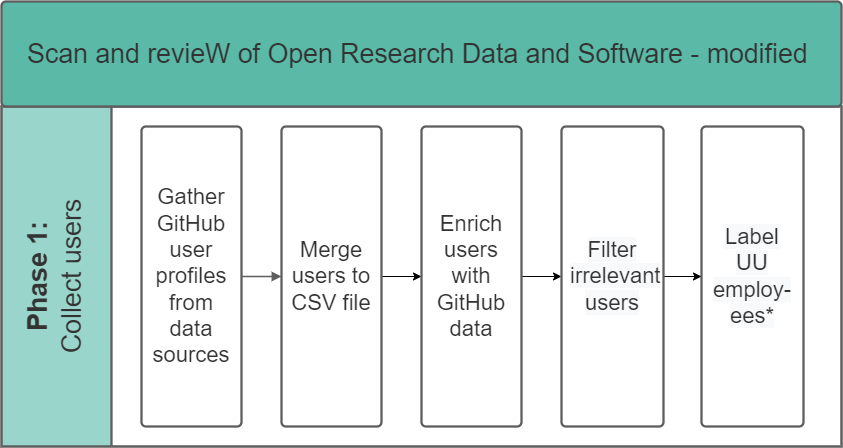
\includegraphics[scale=0.48]{figures/SWORDS-thesis-phase1.drawio.png}
\caption{The modified first phase of the \acrshort{swordsuu} framework. Users are collected, filtered and labelled \cite{de_Bruin_Scan_and_revieW_2021}. 
\label{fig:phase1}}
\end{figure}

The collected users of the steps and search strategies can be seen in \autoref{fig:phase1-method}. All users that were retrieved from the different search strategies during the first step were merged, which left us with 628 unique users. From these, we filtered out 428 irrelevant users, which resulted in 176 identified GitHub users employed at \acrshort{uu}.


\begin{figure}[h!]
\centering
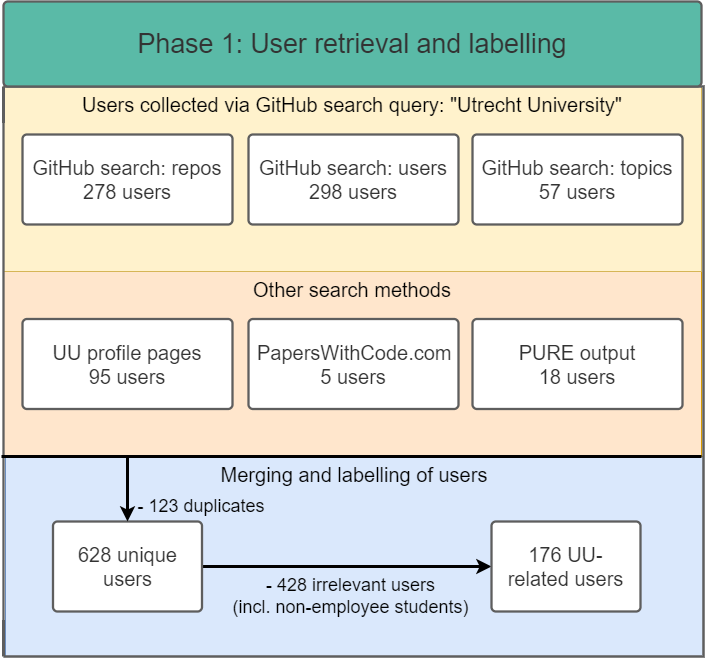
\includegraphics[scale=0.50]{figures/SWORDS-thesis-phase1_method_numbers.drawio.png}
\caption{Results of the non-modified SWORDS pipeline for phase one. 
\label{fig:phase1-method}}
\end{figure}

The 176 \acrshort{uu}-related users are further explained in \autoref{fig:phase1-results}.
Automatic labelling based on provided GitHub metadata and information from the employee pages labelled 129 out of 176 users that needed to be manually verified. The remaining users and the organizations were manually labelled. This process is time sensitive as employees leave and join the university at any given time. The users were collected and labelled during the first two weeks of July 2022. Therefore, this process is naturally not utterly reproducible due to the external API dependency.


\begin{figure}[h!]
\centering
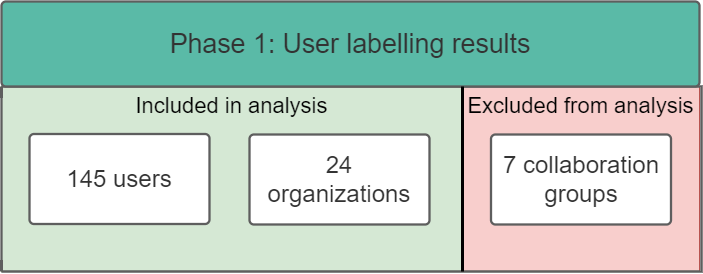
\includegraphics[scale=0.45]{figures/SWORDS-thesis-phase1_results.drawio.png}
\caption{Results of the user labelling for phase one.
\label{fig:phase1-results}}
\end{figure}

\newpage
\subsection{Repository collection}

In phase two, the repositories were collected from the users that were the output of phase one. The complete phase two that was adjusted for this study can be seen in \autoref{fig:phase2}. Filtering consisted of automated filtering of forks and GitHub.io repositories. Forks are copied repositories that are usually used to create pull requests for the original repository. GitHub.io repositories are usually used for documentation or personal websites and not software. Filtering non-research software projects is highly important since most repositories are personal \cite{cosentino_systematic_2017, kalliamvakou_promises_2014}. 
Manual labelling of remaining repositories followed afterwards. The repositories were collected on 18.07.2022 and subsequently labelled until 10.08.2022. This was done in alphabetical order based on username first and repository name second in two iterations, where unclear repositories were left to the second iteration. An overview of the used repository type labels can be found in \autoref{AppendixB}. 
This left us with 823 research-related repositories and 698 non-research-related repositories that are kept for comparison and classification. 

\begin{figure}[h!]
\centering
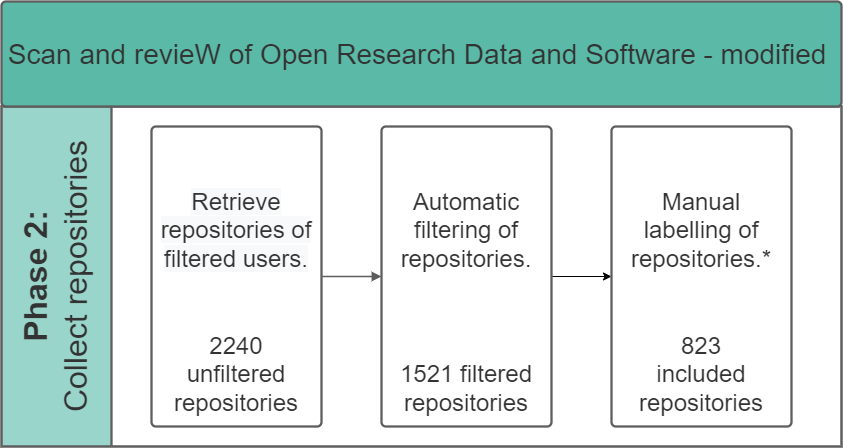
\includegraphics[scale=0.45]{figures/SWORDS-thesis-phase2.drawio.png}
\caption{The modified second phase of the \acrshort{swordsuu} framework. Repositories from identified users are collected, filtered and labelled \cite{de_Bruin_Scan_and_revieW_2021}.
\label{fig:phase2}}
\end{figure}
In addition to the repository type labelling, we also labelled each repository with the corresponding faculty, which is determined by the owner of the repository. There are seven faculties and two support departments:
\begin{itemize}
    \item Faculty of Geosciences
    \item Faculty of Humanities
    \item Faculty of Law, Economics and Governance
    \item Faculty of Medicine
    \item Faculty of Science
    \item Faculty of Social and Behavioural Sciences
    \item Faculty of Veterinary Medicine
    \item University Corporate Offices
    \item Utrecht University Library
\end{itemize}
For labelling, manual verification is always needed. As this study only considered research related to \acrshort{uu}, it was necessary to find out during what time period an employee was employed if the repositories might have been developed at another organization. As such, repositories that were developed before or after employment at \acrshort{uu} were filtered out to the best of available knowledge, e.g. added CVs on employee pages or personal websites. Also, it was required to understand the researchers' subject to better differentiate between research-related and non-research-related projects.

TNO \cite{tno_about}, an independent research organisation, was not treated as a different entity since researchers can be employed at both TNO and UU. Therefore, being an employee of TNO does not exclude a user from our dataset. Even after extensive investigation, some repositories were unclear whether they could be considered research-related or not. In these cases, the author was contacted to clarify, and all requests were answered. In total, this concerned only six users and ten repositories.
For some repositories, it was not possible to clearly distinguish between the labels \textit{non-rs, student work, and irrelevant}, as they are not mutually exclusive. However, that is not an issue since further analysis mostly excluded them, and classification only considers whether a repository is research software or not.



 

\subsection{Variable collection}
In phase three, the howfairis variables, nested GitHub variables, and additional \acrshort{fair} variables were collected. The complete phase three that was adjusted for this study can be seen in \autoref{fig:phase3}.
The howfairis variables were created to check the compliance with the \acrshort{fair} recommendations from the Netherlands eScience Center and DANS \cite{noauthor_fair_nodate}. While the first four variables are related to FAIRness, the \textit{has checklist} variable attempts to cover related topics, such as software engineering best practices. The variable only checks for one very extensive checklist, which might not be appropriate for all kinds of research software \cite{noauthor_badgeapp_nodate}.
Nested variables include information about contributors, used (programming) languages, repository topics, and the README's content. These were collected in separate datasets to achieve a tidy data structure. 
Additional \acrshort{fair} variables that were computed based on available GitHub variables were identified with the help of Martinez et al. \cite{martinez_survey_2022, Spaaks_howfairis} and related GitHub analyses \cite{hasselbring_open_2020, russell_large-scale_2018, pico_fairsoft_2022} and can be seen in \autoref{tab:var}, together with the howfairis variables. For determining to which \acrshort{fair} principle a variable relates to, we considered a combination of the principles by Lamprecht et al. \cite{lamprecht_towards_2020} and Chue Hong et al. \cite{chue_hong_fair_2022} that can be seen in \autoref{AppendixA}. The additional step \textit{Gather and compute additional \acrshort{fair} variables} was incorporated into the \acrshort{swordsuu} framework. The variables were gathered on 12.08.2022 and 13.08.2022.

\begin{figure}[h!]
\centering
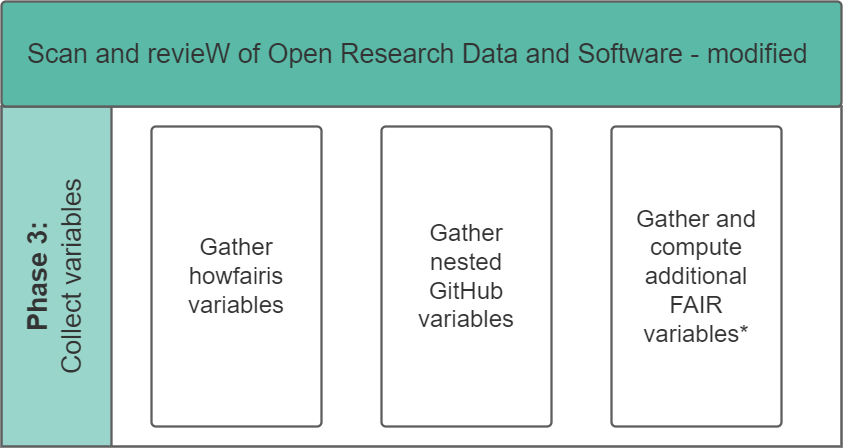
\includegraphics[scale=0.4]{figures/SWORDS-thesis-phase3.drawio.png}
\caption{The modified third phase of the \acrshort{swordsuu} framework. Variables from identified repositories are collected and computed \cite{de_Bruin_Scan_and_revieW_2021}.
\label{fig:phase3}}
\vspace{-0.2cm}
\end{figure}

The howfairis tool outputs five binary \acrshort{fair} variables. \autoref{tab:var} also describes the additional \acrshort{fair} variables that were gathered based on existing literature. These were not part of the \acrshort{swordsuu} data collection yet and were incorporated into \acrshort{swordsuu} as part of this study. The \acrshort{fair} variables from Russell et al. \cite{russell_large-scale_2018} and Hasselbring et al. \cite{hasselbring_open_2020} should serve as a proxy to measure the FAIRness of the repositories. They are about openness and sustainability, which are related to the \acrshort{fair} principles. For the \acrshort{fair} variables from Pico et al. \cite{pico_fairsoft_2022}, we consider incorporating the ones that are applicable to only GitHub data. Many indicators are always valid for GitHub data and, therefore, are not applicable. The implementation of metrics retrieval also differs from the implementation of the references since the quality of these can be improved. As an example, the \textit{version control usage} by Pico et al. only counts versioning with the form of X.X as valid. This does not include semantic versioning, which has the form of X.X.X \cite{preston2013semantic}.
In addition to the \acrshort{fair} variables, we included the metrics in \autoref{tab:metrics} for data analysis. Each metric represents the natural count of occurrences unless otherwise described. Life span is also considered a metric since it is a numeric variable. We also take a deeper look at the license, languages, and topics. 




\afterpage{
{\setlength\LTleft{-1.25cm}
\setlength\LTright{-1cm}
% \scriptsize
\begin{longtable}{@{\extracolsep{\fill}} p{3cm}   p{12.7cm}  p{1.3cm}}
\textbf{Name} & \textbf{Description} & \textbf{FAIR}\\
\hline
\hline
Repository open? & Is the repository open \cite{Spaaks_howfairis}? & F \\
\hline
Has license? & Is there a license \cite{Spaaks_howfairis}? & R \\
\hline
Is registered? & Is the repository registered in a registry \cite{Spaaks_howfairis}? & FI \\
\hline
Has citation? & Is there citation information \cite{Spaaks_howfairis}? & R \\
\hline
Has checklist? & Is there a checklist\footnote{The used version (0.14.1) only checks for the OpenSSF Best Practices checklist} \cite{Spaaks_howfairis}? & FAIR \\
\hline
Correct vcs usage? & Does the repository use version control correctly? This is measured by whether the repository's first and last commit are on the same day \cite{russell_large-scale_2018}. & RS \\
\hline
Life span & The length of time between the first and last commit activity \cite{russell_large-scale_2018, hasselbring_open_2020}. Not considered as FAIR variable but as an additional metric. See \autoref{tab:metrics}. & S \\
\hline
Repository active? & Was there a commit within the last 365 days  \cite{hasselbring_open_2020}? & F \\
\hline
Has install instructions? & Are there installation instructions available \cite{pico_fairsoft_2022}? Checked by mentions of \textbf{install} or \textbf{Docker} in the README file. & R \\
\hline
Has example usage? & Are there examples available \cite{pico_fairsoft_2022}? Checked by mentions of \textbf{usage, getting started, quick start, example, tutorial} in the README file. & R \\
\hline
Has contribution guidelines? & Are there contribution guidelines available \cite{pico_fairsoft_2022}? Checked by mention of \textbf{contribut} in the README file. & A \\
\hline
Has tests? & Is there a tests folder available \cite{pico_fairsoft_2022}? & R \\
\hline
Version identifiable? & Is there a scheme to uniquely and properly identify the software version \cite{pico_fairsoft_2022}? Valid schemes have the form of \textbf{X.X} or \textbf{X.X.X}. & F \\
\hline

\caption{Identified variables with descriptions. The \acrshort{fair} column explains to which principles the variable is related to. S stands for sustainability. Except for life span, all variables are binary. \label{tab:var}}
\end{longtable}}
}



\afterpage{
{\setlength\LTleft{-1.25cm}
\setlength\LTright{-1cm}
% \scriptsize
\footnotesize
\begin{longtable}{@{\extracolsep{\fill}} p{2.7cm}   p{16cm}}
\textbf{Name} & \textbf{Description} \\
\hline
\hline
Stargazers & Represents the number of people that have starred a Github project. Starring a project can indicate that a user likes the project. It can also be used to bookmark a project, since starred projects are saved. The amount of stargazers can be used as a metric to measure popularity. \\ \hline
Issues & A way to keep track of the tasks, enhancements and bugs of the project. They can be discussed in a thread by users and developers. Each repository can enable their own issue page. An issue can be open, for example when a new bug is found, or closed, when it is solved. This shows the amount of open issues a repository has. \\ \hline
Forks & A fork is a copy of a repository for another user. \\ \hline
Size (in MB) & The size of a repository in MB. \\ \hline
Contributors & Contributors refers to the users that have contributed to a repository via commits and pull requests. The number of contributors gives information on how many people put effort into the repository. \\ \hline
Languages & Languages refers to the used languages in a repository. These can be programming languages, markup languages, shell scripts and more. \\ \hline
Topics & Topics refer to the topics a repository is associated with. These are self-assigned. \\ \hline
Life span (in days) & Life span refers to the time between the first and last commit in days. \\ \hline

\caption{Used metrics with descriptions. \label{tab:metrics}}
\end{longtable}}
}


\section{Data analysis}
\label{sec:dataexplore}
To validate subquestion 2, we looked at the Jaccard similarity coefficient \cite{kosub_note_2016} of the howfairis and new \acrshort{fair} variables derived from literature and their percentages for research and non-research software. 
In our case, Jaccard similarity measures pairwise how many of the \acrshort{fair} variables in two repositories are equal and how many are different. It is, therefore, an appropriate measurement for boolean variables. 
The assumption here is that there should be a high similarity to existing \acrshort{fair} variables if they are suitable supplementary variables. This is the preferred measurement over the usual correlation since these variables are all binary. The life span was excluded for this part as it is a metric. We also computed descriptive statistics of the metrics to help answer subquestions 3 and 4: this included minimum, maximum, mean, median, skewness, and kurtosis. Additionally, we looked at the descriptive statistics of metrics, details of \acrshort{fair} variables, and details of license, language, and topic usage for each faculty. A \acrshort{fair} score is computed based on available \acrshort{fair} variables. This is used as a proxy for quantifiable metrics, as most of the variables are binary and therefore not metrics.

For subquestion 3, we additionally conducted multiple univariate Kruskal-Wallis tests with applicable variables, which are all metrics, followed by a post hoc analysis with Dunn's tests. 
The Kruskal-Wallis test represents the non-parametric alternative for one-way \acrfull{anova}. 
An \acrshort{anova} tests equality of means, while a Kruskal-Wallis test compares mean ranks. It is a more general test and less powerful. However, \acrshort{anova} assumes normal-distribution, which our variables do not fulfill. The Dunn’s test compares the mean of each group pairwise and calculates which groups are significantly different.
An alternative approach would be to use a non-parametric multivariate analysis of variance, of which multiple methods exist \cite{anderson_new_2001, katz_multivariate_1980}. There are different justifications for choosing either approach, and they address different research questions \cite{huberty_multivariate_1989}. Some drawbacks are that multiple univariate tests ignore the increased precision of pooled variance estimates, decreasing inference reliability, and the estimation of the correlated error structure, which a multivariate model takes into account \cite{alexis_answer_2015}. However, as it is of interest to us in which metrics the differences exist, a multiple univariate approach is more applicable. Huberty and Morris \cite{huberty_multivariate_1989} also mention that multiple univariate analysis is applicable for exploratory research.

Subquestion 5 was answered with the help of two machine learning model classifications: \textit{logistic lasso regression} and \textit{random forest}. These were trained and tested on 80\% and 20\% of the data, respectively. The models included all metrics and \acrshort{fair} variables. Metrics were scaled to values between zero and one. This allowed us to draw comparisons between variables from the logistic regression coefficients, as all variables are now on the same scale. We used the Python package scikit-learn \cite{scikit-learn} for this part of the analysis.
For describing the models, we will use the term \textit{features} for independent variables and \textit{class} for the categorization of whether a repository is considered research software or not.
We further excluded the feature \textit{repository open}, as this should usually be true for all collected repositories. However, some repositories were either deleted or changed to private between the repository and variable collection, leading to some repositories having a non-true value. These were also excluded from the classification.
We looked at feature importances to determine the most useful ones for each model. Feature importance for logistic regression is measured by coefficients. For random forest, it is measured by permutation feature importance. An alternative measure would be impurity-based feature importance. However, this method is biased towards high cardinality features, which we try to avoid. Additionally, we measured the models with the performance measures accuracy, precision, recall, and F1-score. We compared the scores with a majority class prediction which we named \textit{chance}.


A common topic for consideration while working with generalized linear models, which include logistic regression, is multicollinearity. This refers to the features in such a model having a high correlation. Multicollinearity leads to more unreliable estimates of the coefficients. A common way to address this is by inspecting whether the \acrfull{vif} has a value below five \cite{akinwande_variance_2015}. \autoref{tab:vif} shows that none of the features have a \acrshort{vif} above five.
%
The logistic lasso regression is capable of handling highly correlated features by shrinking coefficients of these towards zero, effectively serving as a feature selection. Logistic lasso regression, as implemented by scikit-learn \cite{scikit-learn}, has one hyperparameter \textit{C} that was tuned via cross-validated randomized search with accuracy as the scoring function. This hyperparameter serves as an inverse of the regularization term, effectively determining the strength of the regularization. A low value equals high regularization, while a large value effectively equals no regularization. As such, we used a randomized search in a log uniform distribution on the training data, ranging from 0.00001 to 100 with 500 iterations, which can be seen in \autoref{fig:randomizedsearch}. This lead us to choose a C-value of 2.545. 

\begin{table}
\centering
\caption{Variance inflation factor values}
\label{tab:vif}
\begin{tabular}{lc}
\toprule
               Variable &  VIF \\
\midrule
       stargazers\_count & 3.87 \\
            open\_issues & 2.15 \\
                  forks & 4.46 \\
                   size & 1.23 \\
     contributors\_count & 3.29 \\
        languages\_count & 2.63 \\
           topics\_count & 1.56 \\
              life\_span & 2.36 \\
      howfairis\_license & 2.19 \\
     howfairis\_registry & 1.41 \\
     howfairis\_citation & 1.42 \\
    howfairis\_checklist & 1.16 \\
              vcs\_usage & 1.10 \\
            repo\_active & 1.69 \\
has\_install\_instruction & 2.06 \\
     has\_usage\_examples & 1.76 \\
 has\_contrib\_guidelines & 1.31 \\
               has\_test & 1.70 \\
   version\_identifiable & 1.74 \\
\bottomrule
\end{tabular}
\end{table}


\begin{figure}[h!]
\centerline{
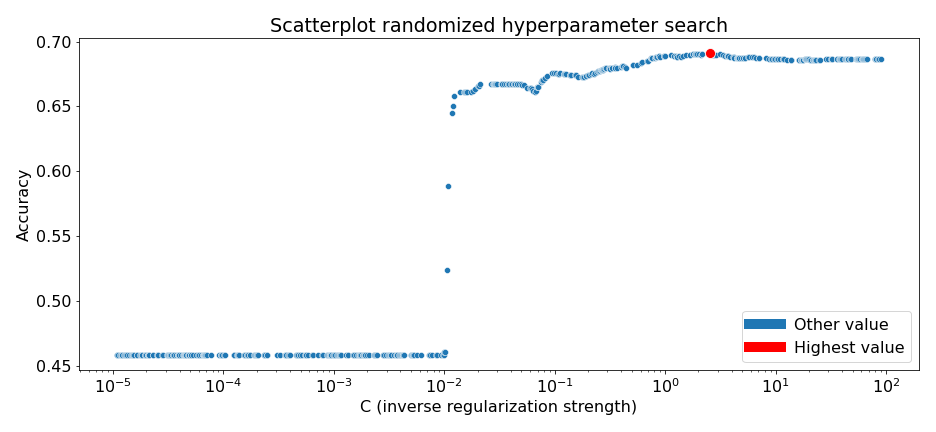
\includegraphics[scale=0.5]{figures_results/stats_scatter_randomsearch_logit.png}}
\caption{Results of the randomized search with a loguniform distribution for values from 0.00001 to 100 and accuracy as the performance evaluation metric.
\label{fig:randomizedsearch}}
\end{figure}

The random forest model had two hyperparameters that were considered for grid search tuning: \textit{maximum number of features} and \textit{number of trees}. While there are many more possible hyperparameters to tune, the default tends to do well for many cases. The grid search concluded with the maximum number of features being the number of all features and a maximum number of trees being 500, which was the maximum search value.

\newpage
\section{Validity}
\label{sec:valid}
There were several threats concerning the study. 
Contributions to research software that \acrshort{uu}-affiliated users do not own are not captured. This means we could not capture if a researcher would contribute to existing open research software. 
The user search process may be flawed, resulting in a biased capture of \acrshort{uu} employees. 
A sole focus on GitHub data may also lead to a similar bias in the data. However, existing literature indicated that this is negligible. 
The used howfairis tool \cite{Spaaks_howfairis} also has flaws. Registering a repository in a registry or having a checklist is not appropriate for all kinds of research software. Especially the checklist can often be too convoluted for simple research software, such as research scripts.
Due to the amount of captured repositories, manual labelling of these might also be error-prone, especially considering the opinionated discussions regarding the definition of what qualifies as research software \cite{gruenpeter_defining_2021}. The daily supervisor Jonathan de Bruin reviewed the created labels to minimise possible mislabelling. However, a more significant threat to any GitHub analysis validity would be to include personal use repositories \cite{kalliamvakou_promises_2014}, as they are not the focus of this study. 

These threats are an inherent part of the method used. Nonetheless, the results benefit academia, as stated in \autoref{chap:intro}. The findings help to improve the \acrshort{rse} practice with concrete recommendations and novel findings. The method can also be adapted for other organizations as it is publicly available \cite{Quach_Mapping-Research-Software-Landscapes-through-Exploratory-Studies-of-GitHub-Data_2022} and thus lays the groundwork for similar studies that may also improve the proposed method. Additionally, the created dataset will be openly shared for others to reuse.





